\documentclass[a4paper,10pt]{article}
\usepackage[brazilian]{babel}
\usepackage[T1]{fontenc}
\usepackage[utf8]{inputenc}
\usepackage{lmodern}
\usepackage{geometry}
\geometry{verbose,tmargin=3cm,bmargin=3cm,lmargin=2cm,rmargin=2cm}
\usepackage{fancyhdr}
\pagestyle{fancy}
\usepackage{amsthm}
\usepackage{amsmath}
%\numberwithin{equation}{section}
\usepackage{amsfonts}
\usepackage{amssymb}
\usepackage{mathtools}
%\usepackage{mnsymbol}
\usepackage[authoryear]{natbib}
\usepackage{algorithm}
\usepackage{algpseudocode}
\usepackage[hyphens]{url}
\usepackage{color}
\usepackage{graphicx}
\usepackage{xcolor}
\usepackage{import}
\usepackage{bm}
\usepackage{cancel}
\usepackage{listings}
\usepackage{graphicx}
\usepackage{caption}
\usepackage{subcaption}
\graphicspath{{Figures/}}

\usepackage{xcolor}

\definecolor{codegreen}{rgb}{0,0.6,0}
\definecolor{codegray}{rgb}{0.5,0.5,0.5}
\definecolor{codepurple}{rgb}{0.58,0,0.82}
\definecolor{backcolour}{rgb}{0.95,0.95,0.92}

\lstdefinestyle{mystyle}{
	backgroundcolor=\color{backcolour},   
	commentstyle=\color{codegreen},
	keywordstyle=\color{magenta},
	numberstyle=\tiny\color{codegray},
	stringstyle=\color{codepurple},
	basicstyle=\ttfamily\footnotesize,
	breakatwhitespace=false,         
	breaklines=true,                 
	captionpos=b,                    
	keepspaces=true,                 
	numbers=left,                    
	numbersep=5pt,                  
	showspaces=false,                
	showstringspaces=false,
	showtabs=false,                  
	tabsize=2
}

\lstset{style=mystyle}

\makeatletter
\usepackage[colorlinks=true,linkcolor=red]{hyperref}
\makeatother




\bibliographystyle{apalike2}

\begin{document}
% ------------------ NOTA -----------------------
%
% 1 - Você não precisa alterar o arquivo de template, somente esse arquivo.
% 2 - Abaixo de cada comando há uma nota que o auxiliará a preencher os campos. Todos os
%     comandos são auto-explicáveis, mas as notas o ajudarão em caso de dúvidas.
%
% -----------------------------------------------

\newcommand{\surname}{RAFFO}
% Substitua "SOBRENOME" por ADORNO, RAFFO ou PIMENTA, conforme quem for o seu orientador.
% No caso de haver um co-orientador, use as três primeiras letras de cada sobrenome separadas
% por '/'. Por exemplo, se seu orientador é o Prof. Adorno e seu co-orientador é o Prof.
% Pimenta, escreva ADO/PIM.

\newcommand{\initials}{JMC}
% Coloque suas iniciais aqui (ex., Bruno Vilhena Adorno = BVA)

\newcommand{\reportnumber}{1}
% Mude "X" pelo número do relatório

\newcommand{\reportversion}{1}
% Mude "Y" pelo número da versão do relatório.

\newcommand{\reporttitle}{\textbf{Parallel Distributed Control(PDC) de um Pendulo Invertido Via Representação Takagi-Sugeno}}

\newcommand{\registrationnumber}{2016086496}

\newcommand{\studentname}{Jonatan Mota Campos}

\newcommand{\advisorname}{Guilherme Vianna Raffo}

\newcommand{\coadvisorname}{}

\newcommand{\macroheader}[4]{MACRO/#1--\the\year /#2/#3+Versão-#4}


\lfoot{\noindent \macroheader{\surname}{\initials}{\reportnumber}{\reportversion}}


\cfoot{}


\rhead{\noindent 
\includegraphics[width=0.15\textwidth]{report_template/macro_inline}}


\rfoot{\thepage}


\lhead{\leftmark}

\thispagestyle{empty}

\noindent \begin{center}
\textbf{}%
\begin{minipage}[t]{1\columnwidth}%
\noindent \begin{center}
\textbf{}%
\begin{minipage}[c]{0.3\columnwidth}%
\noindent \begin{flushleft}

\includegraphics[width=1\textwidth]{report_template/macro_inline_name}
\par\end{flushleft}%
\end{minipage}\textbf{}%
\begin{minipage}[b]{0.7\textwidth}%
\noindent \begin{flushright}
\textbf{\macroheader{\surname}{\initials}{\reportnumber}{\reportversion}}
\par\end{flushright}%
\end{minipage}
\par\end{center}%
\end{minipage}
\par\end{center}

\noindent \rule[0.5ex]{1\textwidth}{1pt}

\bigskip{}


\begin{center}
\textbf{\Large{}Universidade Federal de Minas Gerais - UFMG}
\par\end{center}{\Large \par}

\begin{center}
\textbf{\large{}Programa de Pós-Graduação em Engenharia Elétrica}
\par\end{center}{\large \par}

\vspace{6cm}


\begin{center}
{\LARGE{}\reporttitle}
\par\end{center}{\LARGE \par}

\vfill{}


\textit{\emph{\large{}Número de matrícula: \registrationnumber}}{\large \par}

\textit{\emph{\large{}Estudante: \studentname}}{\large \par}

\textit{\emph{\large{}Orientador: \advisorname}}{\large \par}

\textit{\emph{\large{}Co-orientador: \coadvisorname}}{\large \par}

\vspace{1cm}


\begin{flushright}
\textit{\emph{\today}}
\par\end{flushright}

\pagebreak{}


% % % % % % % % % % % % % % % % % % % % % % % % % % %
\newpage
\tableofcontents
\thispagestyle{empty}

\newpage
\pagenumbering{arabic}
% % % % % % % % % % % % % % % % % % % % % % % % % % %
\newcommand{\zero}{\bm{\emptyset}}

\section{Modelagem Dinâmica}
\subsection{Formulação Newton Euler e Representação Via Sistema Descritor}
\paragraph{} Pela modelagem de Newton Euler, que não será demonstrada aqui por ja ter sido demonstrada no arquivo fornecido para o trabalho obtêm-se o modelo dinâmico abaixo:
\begin{gather}
	\begin{bmatrix}
		M+m & -mlcos(\theta) \\
		-mlcos(\theta) & ml^2
	\end{bmatrix}\begin{bmatrix}
	\ddot{s} \\ \ddot{\theta}
\end{bmatrix} + \begin{bmatrix}
0 & mlsin(\theta) \\
0 & 0
\end{bmatrix}\begin{bmatrix}
\dot{s} \\ \dot{\theta}
\end{bmatrix} + \begin{bmatrix}
(M+m)gsin(\alpha) \\
-mglsin(\alpha+\theta)
\end{bmatrix} = \begin{bmatrix}
u - k_v\dot{s} \\
0
\end{bmatrix}
\end{gather}
\paragraph{}Onde, $M$ é a massa do carrinho, $m$ é a massa do pendulo, $g$ é a aceleração da gravidade, $l$ é a distancia entre o centro de gravidade do pendulo e seu eixo de rotação, $s$ é a distância percorrida pelo carrinho, $\theta$ é a incliinação do pendulo, e $k_v$ é uma constante de atrito viscoso.
\begin{figure}[h]
	\centering
	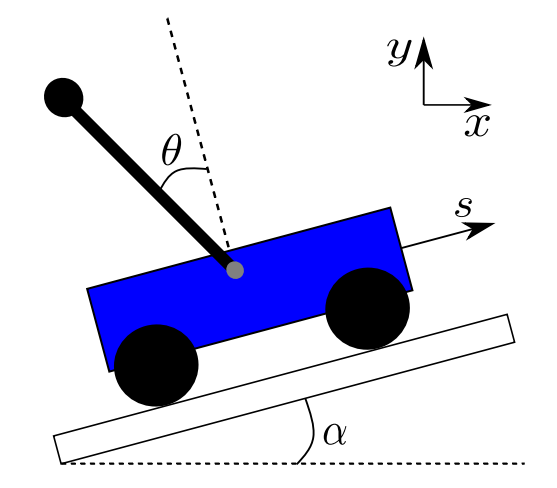
\includegraphics[scale=0.5]{fig/pendulo}
	\caption{Pêndulo Invertido}
\end{figure}
\paragraph{}Definindo ainda $v = \dot{s}$ e $\omega = \dot{\theta}$ escreve-se a dinâmica em malha aberta como,
\begin{gather}
	\begin{split}
			\begin{bmatrix}
			1 & 0 & 0 & 0 \\
			0 & 1 & 0 & 0 \\
			0 & 0 & M+m & -mlcos(\theta) \\
			0 & 0 & -mlcos(\theta) & ml^2
		\end{bmatrix}\begin{bmatrix}
			\dot{s} \\ \dot{\theta} \\ \dot{v} \\ \dot{\omega}
		\end{bmatrix} = \begin{bmatrix}
			0 & 0 & 1 & 0 \\
			0 & 0 & 0 & 1 \\
			0 & 0 & -k_v & -mlsin(\theta)\omega \\
			0 & mglcos(\alpha)sinc(\theta) & 0 & 0
		\end{bmatrix}\begin{bmatrix}
			s \\ \theta \\ v \\ \omega
		\end{bmatrix} \\
	+ \begin{bmatrix}
		0 \\ 0 \\ 1 \\ 0
	\end{bmatrix}u + \begin{bmatrix}
	0 \\ 0 \\ -(M+m)gsinc(\alpha) \\ mglcos(\theta)sinc(\alpha)
\end{bmatrix}\alpha
	\end{split}
\end{gather}
\paragraph{} Fazendo $\bar{\alpha} = sinc(\alpha)\alpha$ escreve-se o sistema descritor quasi-LPV como,
\begin{gather}
	\bm{E}(x)\dot{\bm{x}} = \bm{A}(x)\bm{x} + \bm{B_u}u + \bm{B_\alpha}(x)\bar{\alpha} \\
		\begin{split}
		\begin{bmatrix}
			1 & 0 & 0 & 0 \\
			0 & 1 & 0 & 0 \\
			0 & 0 & M+m & -mlcos(\theta) \\
			0 & 0 & -mlcos(\theta) & ml^2
		\end{bmatrix}\begin{bmatrix}
			\dot{s} \\ \dot{\theta} \\ \dot{v} \\ \dot{\omega}
		\end{bmatrix} = \begin{bmatrix}
			0 & 0 & 1 & 0 \\
			0 & 0 & 0 & 1 \\
			0 & 0 & -k_v & -mlsin(\theta)\omega \\
			0 & mglcos(\alpha)sinc(\theta) & 0 & 0
		\end{bmatrix}\begin{bmatrix}
			s \\ \theta \\ v \\ \omega
		\end{bmatrix} \\
		+ \begin{bmatrix}
			0 \\ 0 \\ 1 \\ 0
		\end{bmatrix}u + \begin{bmatrix}
			0 \\ 0 \\ -(M+m)g \\ mglcos(\theta)
		\end{bmatrix}\bar{\alpha}
	\end{split}
\end{gather}


\subsection{Representação Takagi-Sugeno Via Não Linearidade de Setor}
\paragraph{}Nessa seção será utilizada a técnica de não linearidade de setor para buscar um modelo Takagi-Sugeno exato dentro de um domínio compacto. São escolhidas as seguintes não linearidades:
\begin{gather}
	\begin{cases}
		z_1 = cos(\theta) \\
		z_2 = sin(\theta)\omega \\
		z_3 = cos(\alpha)sinc(\theta)
	\end{cases}
\end{gather}
 \paragraph{}Dessa forma obtemos um modelo dinâmico na forma,
 \begin{gather}
 %	\dot{\hat{\bm{x}}} = \bm{f(x)}\bm{x} + \bm{B_u}u + \bm{g(x)}\bar{\alpha} \\
 	 	\dot{\bm{x}} =  
 	 	\Biggl\{\begin{bmatrix}
 	 		1 & 0 & 0 & 0 \\
 	 		0 & 1 & 0 & 0 \\
 	 		0 & 0 & M+m & -mlcos(\theta) \\
 	 		0 & 0 & -mlcos(\theta) & ml^2
 	 	\end{bmatrix}\Biggr\}^{-1}	\Biggl\{\begin{bmatrix}
 			0 & 0 & 1 & 0 \\
 			0 & 0 & 0 & 1 \\
 			0 & 0 & -k_v & -mlz_2 \\
 			0 & mglz_3 & 0 & 0
 		\end{bmatrix}\begin{bmatrix}
 			s \\ \theta \\ v \\ \omega
 		\end{bmatrix} 
 		+ \begin{bmatrix}
 			0 \\ 0 \\ 1 \\ 0
 		\end{bmatrix}u + \begin{bmatrix}
 			0 \\ 0 \\ -(M+m)g \\ mglz_1
 		\end{bmatrix}\bar{\alpha}	\Biggl\} \\
 	\dot{\bm{x}} = \bm{f(\bm{x},\bm{u},\bm{\hat{\alpha}})}
 \end{gather}
\paragraph{} Como $\dot{\bm{x}} = \bm{f(0,0,0)} = 0$ podemos utilizar a técnica da não linearidade de setor. Tomando a condição de que estamos projetando um controlador para atuar em um terreno com inclinação máxima e minima conhecidas de forma que $\alpha \in$ [-10\textdegree ,10\textdegree], além de que da geometria do problema $\theta \in$ [-90\textdegree ,90\textdegree], e assumindo que a velocidade angular do pendulo varie como $\omega \in$ [-$\frac{pi}{6}(\frac{rad}{s})$ ,$\frac{pi}{6}(\frac{rad}{s})$].


\noindent \begin{minipage}{.25 \linewidth}
\begin{gather}
	a_{1}^{max} = 1 \\
	a_{1}^{min} = 0 \\	
\end{gather}
\end{minipage}
\hfill
 \begin{minipage}{.25 \linewidth}
	\begin{gather}
		a_{2}^{max} = 0.5236 \\
		a_{2}^{min} = -0.5236 \\	
	\end{gather}
\end{minipage}
\section{Controle}
\subsection{Lei de Controle PDC}
\subsection{Lei de Controle PDC com $\mathcal{H}_\infty$}



\end{document}
